\begin{center}\textsc{Gauss} an \textsc{Olbers}.\quad Göttingen, 14. Mai 1826.\end{center}

.\ .\ .\ .\ .\ .\ Ich bin eine beträchtliche Zeit mit der Ausgleichung meines
Winkelsystems beschäftigt gewesen, eine, weil ich alle Willkür ausschliessen
wollte, sehr beschwerliche Arbeit, da dabei alles unter einander zusammenhängt,
und gewissermaassen die Messungen in Jever auf die in Göttingen
reagiren. Es hat vielleicht noch niemals jemand eine so complicirte Elimination
ausgeführt, wo 55 Gleichungen ebenso viele unbekannte Grössen involvirten.
Heute bin ich damit fertig geworden, so dass nun alle 150 Richtungen,
die das System enthält, so ausgeglichen sind, mit den möglich kleinsten
Änderungen, dass sie genau mit einander harmoniren. Es sind unter den
150 fünf, die über $1^{\prime\prime}$ haben geändert werden müssen (die grössten $1^{\prime\prime}{,}373$,
nemlich Garlste-Varel und Varel-Garlste), und der sogenannte mittlere Richtungsfehler
wird $0^{\prime\prime}{,}755$, viel grösser, als nach der schönen Übereinstimmung
der Messungen auf jeder Station unter sich, zulässig ist, so dass ich das
Dasein der Lateral-Refraction in den flachen Gegenden gar nicht bezweifeln
kann; in den höhern Gegenden sind die Ausgleichungen immer viel kleiner. ---

Es war eine langweilige Arbeit, alle Messungen erst genau vorzubereiten,
da ich nichts vernachlässigen wollte, und die kleinen Reductionen der Consequenz
wegen doch überall zugezogen werden sollten. \textsc{Bessel} hat, so viel ich
weiss, zuerst öffentlich von derjenigen gesprochen, die daher rührt, dass der
Winkel der kürzesten Linie von dem Winkel der Verticalebene differirt; allein
er hat dabei bloss die Punkte als auf der Oberfläche des Sphäroids betrachtet:
\clearpage
\noindent\textbf{ZUR NETZAUSGLEICHUNG.}\hfill321\par\medskip
\noindent meistens beträgt diese Reduction nur ein Paar Tausendtheile einer Secunde;
wollte ich sie aber einmal zuziehen, so durfte ich eine andere nicht übergehen,
die gewöhnlich viel grösser (obgleich auch noch unbedeutend) ist, und
daher rührt, dass die Punkte, die in Einer Verticallinie liegen, nicht in Einer
Verticalebene erscheinen, so dass eine von der Höhe abhängige Reduction
hervorgeht. Diese hat immer das entgegengesetzte Zeichen von \textsc{Bessels} Correction
und ist schon bei mässigen Höhen immer grösser, oft 4-mal, 8-mal
so gross, so dass jene immer destruirt und weit überflügelt wird. Der grösste
Betrag in meinem System ist von Lichtenberg zum Brocken, wo er $-0^{\prime\prime}{,}041$
ausmacht. --- Die genaue Berechnung der 51 Dreiecke selbst wird jetzt ein
leichtes Spiel sein.
\par\medskip
.\ .\ .\ .\ .\ .

Ich habe mich heute noch etwas in dem System der \textsc{Krayenhoff}schen
Dreiecke im Innern von Holland umgesehen. Ich sehe immer mehr, wie
wenig ich Ursache habe, mich über meinen grössten Richtungsfehler von $1^{\prime\prime}{,}4$
zu beunruhigen. Wenn man \textsc{Krayenhoffs} Messungen oberflächlich prüft, d.\ i.\
die Summen der 3 Dreieckswinkel und den Gyrus horizontis, so findet man
überall so schöne Übereinstimmung, dass man verleitet wird, diesen Messungen
eine Genauigkeit beizulegen, von der sie doch \textls[120]{sehr} weit entfernt sind. Nichts
ist dazu zweckmässiger als die Verbindungen von mehr als 3 Punkten, die
verknüpfte Dreiecke geben. Hier findet man häufig viel grössere Differenzen.
\begin{center}
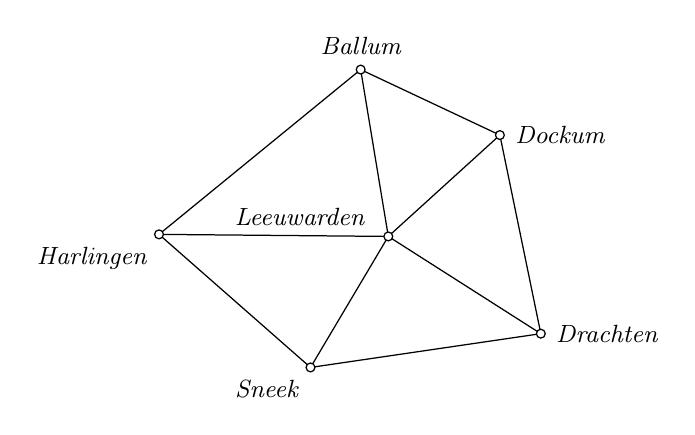
\begin{tikzpicture}[x=1.3cm,y=1.3cm,line width=.45pt,font=\small\itshape]
\coordinate (H) at (0,1.30);
\coordinate (B) at (1.97,2.91);
\coordinate (D) at (3.33,2.27);
\coordinate (R) at (3.73,.33);
\coordinate (S) at (1.48,0);
\coordinate (L) at (2.24,1.28);
\draw (H)--(B)--(D)--(R)--(S)--cycle;
\draw (L)--(H) (L)--(B) (L)--(D) (L)--(R) (L)--(S);
\foreach \p in {H,B,D,R,S,L}{\draw[fill=white] (\p) circle[radius=1.6pt];}
\node[above=2pt] at (B) {Ballum};
\node[right=2pt] at (D) {Dockum};
\node[right=2pt] at (R) {Drachten};
\node[below left=1pt] at (S) {Sneek};
\node[below left=1pt] at (H) {Harlingen};
\node[anchor=east,xshift=-.18cm,yshift=.25cm] at (L) {Leeuwarden};
\end{tikzpicture}
\end{center}
\begingroup
\makeatletter
\renewcommand{\@makefnmark}{\hbox{\normalfont[\textsuperscript{*})]}}
\renewcommand{\@makefntext}[1]{\parindent1em\noindent\hbox to1.8em{\hss[\textsuperscript{*})\ }#1]}
\makeatother
\noindent Z.\ B.\ das System von 6 Punkten\footnote{Vergl. Band IV, S.\ 82/87.} gibt den Gyrus horizontis von Leeuwarden
vortrefflich, auf $2^{\prime\prime}{,}197$ genau; die Summen der Winkel in den 5 Dreiecken
fehlen resp.
\[
\begin{array}{r}
1^{\prime\prime}{,}432\\
0{,}714\\
0{,}759\\
2{,}842\\
2{,}590,
\end{array}
\]
\endgroup
\makeatletter
\def\ps@gaussIXfortyone{\def\@oddhead{}\def\@evenhead{}\def\@oddfoot{\small IX.\hfil41}\let\@evenfoot\@oddfoot}
\makeatother
\thispagestyle{gaussIXfortyone}
\clearpage
\noindent322\hfill\textbf{BRIEFWECHSEL.}\par\medskip
\begingroup
\makeatletter
\renewcommand{\@makefnmark}{\hbox{\normalfont\textsuperscript{*})}}
\makeatother
\noindent also auch erträglich. Aber wenn man die Seitenverhältnisse prüft, so findet
man, dass die Messungen sich nicht vereinigen lassen, ohne an den 10 Winkeln
in der Peripherie viel grössere Änderungen zu machen; nach der Methode
der kleinsten Quadrate müsste man sie um $3^{\prime\prime}{,}8$, $3^{\prime\prime}{,}6$, $3^{\prime\prime}{,}6$, $3^{\prime\prime}{,}3$, $3^{\prime\prime}{,}0$, $2^{\prime\prime}{,}7$, $2^{\prime\prime}{,}7$,
$1^{\prime\prime}{,}9$, $1^{\prime\prime}{,}1$, $0^{\prime\prime}{,}8$ ändern; wollte man die Änderungen so klein wie möglich haben,
so müsste man sie alle 10 gleich und jede $=3^{\prime\prime}$ setzen\footnote{\textsc{Krayenhoffs} eigene Ausgleichung, die aber nicht klar aufgestellt ist, sondern erst herausgesucht werden muss, enthält hier zum Theil noch viel grössere Änderungen z.\ B.\ von $6^{\prime\prime}{,}253$ an dem einen Winkel in Drachten, $5^{\prime\prime}{,}530$ an einem Winkel in Dockum, etc.}. Man sieht also,
dass bei solchen Messungen die Summe der 3 Dreieckswinkel oft über $10^{\prime\prime}$
fehlen müsste. Davon sind die aufgestellten Zahlen aber weit entfernt, und
also [ist] gewiss, dass wenigstens immer nur so \textls[120]{ausgesucht} ist, dass \textls[120]{diese}
Prüfung harmonirt, wodurch aber offenbar oft geschehen muss, dass die
Winkel eher verdorben als verbessert werden, und ein ganz falscher Maassstab
für ihre Genauigkeit hervorgeht. Um die Genauigkeit von Messungen
gehörig würdigen zu können, darf nichts willkürlich ausgeschlossen werden.
Die leichten Prüfungen durch die Summen der 3 Dreieckswinkel und den
Gyrus horizontis sind wohl gar zu verführerisch, wenn auch nicht gerade zu
verfälschen, doch zum Wählen und Ausschliessen, was nicht viel besser ist.
Leider bieten andere Messungen, wie die von \textsc{Delambre}, sonst fast gar keine
Prüfungen dar, als die erwähnten, sonst möchte man wohl oft ähnliche
Discordanzen finden.

Bei meinem System habe ich die Satisfaction gehabt, dass die Prüfungen
der einen und der andern Art Differenzen geben, die ganz von einerlei Ordnung
sind. Dass die Seitenrefractionen so grosse Wirkungen geben, wie die
Disharmonien, die sich bei \textsc{Krayenhoffs} Dreiecken zeigen, ist mir doch bedenklich,
da seine Seiten immer so klein sind, seine Stationen hoch in der
Luft, und Holland auch wohl viel weniger von Holz coupirt, wie mein nördliches
Terrain, so dass bei ihm das Licht wohl selten oder nie so knapp an
Hindernissen wegstrich, wie so sehr oft in dem letztern. Ich möchte also die
Anomalien eher den Messungen selbst zuschreiben.
\endgroup
